\chapter{Tecnologías}
\label{chap:tecnologias}
A lo largo del capítulo se explicarán las tecnologías utilizadas para la realización del proyecto, así como otros aspectos relacionados con su desarrollo.

\section{Arquitectura}

Para comenzar a desarrollar un proyecto software hay que tener en cuenta qué herramientas vamos a usar y qué requisitos debemos cumplir. Por ello se necesita conocer cómo va a ser la estructura de alto nivel de nuestro proyecto para desarrollarla y de esta manera conseguir un sistema robusto y escalable. 

En este proyecto se ha utilizado una arquitectura de tres capas [Figura \ref{fig:arquitectura}] que se distribuye de la siguiente manera:

\begin{itemize}
    \item \textbf{Capa de Presentación:}  Presenta el sistema al usuario, le comunica la información y captura la información. Esta capa se comunica únicamente con la capa de negocio.    
    \item \textbf{Capa de Negocio:} Se reciben las peticiones del usuario y se envían las respuestas tras la ejecución. Se denomina capa de negocio porque es donde se establecen las reglas de procesado de los datos. Esta capa se comunica con la capa de presentación, para recibir solicitudes y enviar los resultados, y con la capa de datos, para solicitar el almacenamiento y recuperación de los datos.
    
    \item \textbf{Capa de Datos:}  Es donde residen los datos y es la encargada de acceder a los mismos. Está formada por uno o varios gestores de bases de datos que se encargan de procesar las solicitudes de almacenamiento o recuperación de información desde la capa de negocio.

\end{itemize}

Cada una de estas capas suele distribuirse en distintos servidores, aunque podría darse que todas las capas se encontrasen en uno solo. Este tipo de arquitectura permite replicar la capa que más lo necesite. Lo que otorga la capacidad de escalar la aplicación sobre las partes que se consideren más críticas. Es decir, si tenemos un sistema que necesita procesar muchas operaciones de guardado o lectura de datos, podríamos replicar la capa de datos en otros ordenadores balanceando las peticiones sobre los nuevos servicios creados.
\begin{figure}[H]
    \centering
    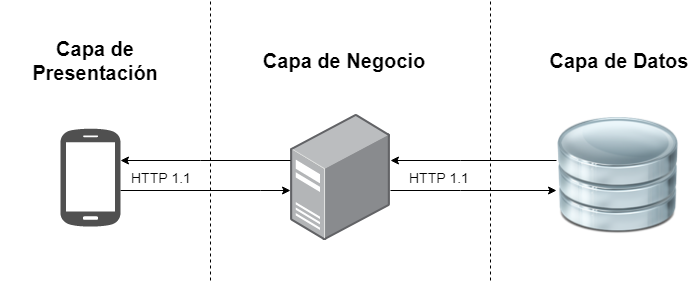
\includegraphics[width=0.7\textwidth, keepaspectratio]{imaxes/layer.png}
    \caption{Arquitectura de tres capas}
    \label{fig:arquitectura}
\end{figure}


\subsection{Capa de Presentación}
Para esta parte de la arquitectura se ha utilizado \textit{Angular} como \textit{framework} de desarrollo principal e \textit{Ionic} y \textit{Capacitor} como para la interfaz visual y creación de una aplicación \textit{Android} respectivamente.

Al desarrollar una aplicación en \textit{Angular} nos vemos forzados a usar el patrón \textit{MVVM} (Modelo-Vista-Vista-Modelo) [Figura \ref{fig:mvvm}], ya que es el utilizado por este \textit{framework}.
Este patrón consiste en la modificación del modelo por parte de la vista y la modificación de la vista por parte del modelo, utilizando la técnica del doble enlace (\textit{two way binding}) implementada por este \textit{framework}.


\begin{figure}[H]
    \centering
    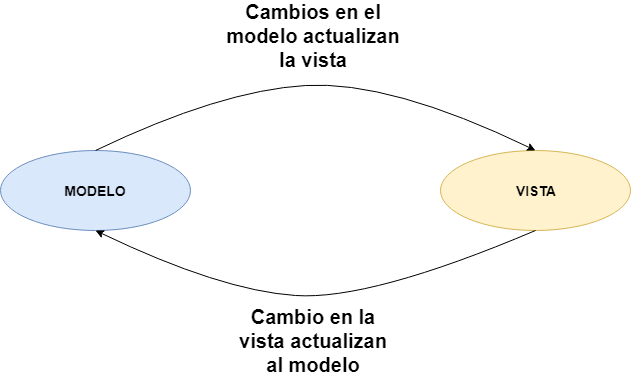
\includegraphics[width=0.6\textwidth, keepaspectratio]{imaxes/MVVM.png}
    \caption{Patrón Modelo-Vista-Vista-Modelo}
    \label{fig:mvvm}
\end{figure}


\subsubsection{Angular~\cite{angular}}
Es un \textit{framework} de desarrollo \textit{Javascript} , creado por Google. Dicho \textit{framework} nos ayuda al desarrollo de aplicaciones web SPA (\textit{Single Page Aplication}).

Se ha decidido utilizar \textit{Angular} por las siguientes razones:
\begin{itemize}
    \item Permite crear aplicaciones modulares y con componentes que pueden ser reutilizables a lo largo de la aplicación, lo que genera un código más limpio y fácil de mantener.
    \item Se integra con bien con \textit{Ionic} para crear aplicaciones híbridas.
    \item Utiliza inyección de dependencias, un patrón que permite instanciar los servicios directamente sin necesidad de crearlos localmente.
    \item Proporciona un programa de línea de comandos que permite generar plantillas para ciertos componentes del código.
    \item Proporciona un conjunto de librerías que facilitan aspectos como la realización de peticiones y envío de datos a través de \textit{HTTP} o navegación entre las páginas de la aplicación.
\end{itemize}

\subsubsection{Ionic~\cite{ionic}}
Es una librería \textit{Javscript} que nos permite construir de manera sencilla y rápida la interfaz de nuestra aplicación.

Se ha decidido usar \textit{Ionic} por las siguientes razones:
\begin{itemize}
    \item Abstrae al diseñador de dibujar los componentes, centrándose en cómo se verán la pantalla.
    \item Permite utilizar la misma interfaz en distintas plataformas, adaptándose automáticamente a estas plataformas (Android, escritorio, web e IOS)
    \item Se integra perfectamente con los \textit{frameworks} más usados del mercado como \textit{Angular}.
    \item Está implementado en su totalidad con componentes web\footnote{Componentes reutilizables que siguen las especificaciones \textit{HTML} y \textit{DOM} establecidas por el \textit{W3C}}, lo que proporciona un rendimiento y compatibilidad mayores.
\end{itemize}

\subsubsection{Capacitor~\cite{capacitor}}
Es una librería \textit{Javascript}, creada por \textit{Ionic}, que contiene una conjunto de herramientas, las cuales nos permiten exportar una aplicación web a una aplicación móvil de manera nativa.

Se ha decidido usar \textit{Capacitor} por las siguientes razones:
\begin{itemize}
    \item Proporciona un desarrollo único para las diferentes plataformas móviles.
    \item Proporciona acceso a los componentes del dispositivo de forma nativa.
    \item Soporte para \textit{plugins} que permiten acceder a nuevas funcionalidades del sistema.
    \item Permite la ejecución de código nativo dentro de la plataforma.

\end{itemize}

\subsubsection{Cypress~\cite{cypress}}

Es un librería \textit{Javascript} que nos permite ejecutar pruebas en aplicaciones web de manera automática, pero pensada para aplicaciones web, ya que dichas pruebas se ejecutan en el navegador y comprueban tanto el correcto funcionamiento de la aplicación como su flujo de ventanas. 

Las ventajas que proporciona \textit{cypress} frente a otras herramientas de pruebas son las siguientes:
\begin{itemize}
    \item Contiene un entorno gráfico que permite una programación más ágil.
    \item Soporta la ejecución de pruebas en cualquier navegador, independientemente del sistema operativo utilizado.
    \item Permite acceder a los elementos que se necesitan probar de una manera sencilla.
\end{itemize}



\subsection{Capa de Negocio}

La capa de lógica de negocio es ejecuta en \textit{NodeJS} y programada en \textit{Typescript} usando para ello el \textit{framework} \textit{NestJS} y otras librerías como: \textit{JWT}, \textit{bcrypt}, \textit{mongoose}\dots~ para autenticicación y conexiones con los servicios.

Adicionalmente, para el desarrollo numérico/computacional se ha usado \textit{Python} y la librería \textit{Sklearn}. 

Se han creado dos servidores [Figura~\ref{fig:servers_schema}] para comunicar ambos lenguajes de programación, donde el servidor de \textit{Python} solo se comunica con el de \textit{Node}, el cual realiza las conexiones al exterior.

\begin{figure}[h]
    \centering
    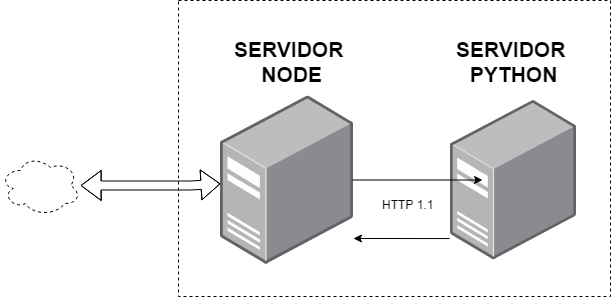
\includegraphics[width=0.6\textwidth, keepaspectratio]{imaxes/servers_schema.png}
    \caption{Capa de lógica de negocio}
    \label{fig:servers_schema}
\end{figure}

\subsubsection{NestJS~\cite{nestjs}}
Es un \textit{framework} de desarrollo para aplicaciones servidor en \textit{NodeJS}. Utiliza Typescript como lenguaje principal de programación y contiene una extensa documentación que abarca la mayor parte de las necesidades requeridas de un servidor.
Las ventajas que proporciona este \textit{framework} son las siguientes:

\begin{itemize}
\item Hace uso de decoradores\footnote{Envolturas que se utilizan sobre funciones, clases\dots~ para añadir más funcionalidad}, lo que supone una programación más ágil, legible y menos propensa a errores.
\item Se integra perfectamente con la mayoría de las herramientas existentes, haciendo que la programación con servicios de terceros funcione correctamente (Base de datos, OpenAPI, Jest~\dots)
\item Utiliza una estructura similar a la usada por \textit{Angular}. Por lo tanto, al usar estos dos \textit{frameworks} en el lado del cliente y el lado del servidor se reduce la complejidad de lectura del código.
\end{itemize}


\subsubsection{Jest~\cite{jest}}

Es un librería \textit{Javascript}, desarrollado por Facebook, que contiene un conjunto de herramientas para ejecutar pruebas de forma automática.

El \textit{framework} de \textit{NestJs} proporciona documentación sobre las pruebas utilizando esta librería, además de ser una de las más usadas en entornos \textit{Javascript}. También proporciona soporte para \textit{Typescript}.

\subsubsection{Sklearn}
\textit{Sklearn}~\cite{sklearn} es una librería de aprendizaje máquina para el lenguaje de programación \textit{Python}.  Se ha usado \textit{Sklearn} por las siguientes razones:
\begin{itemize}
    
\item Se encuentra bien documentada, incluyendo ejemplos para cada función.
\item Mantiene un interfaz consiste ante los distintos modelos de aprendizaje automático.
\item Proporciona funcionalidades adicionales que permiten un desarrollo más ágil.

\end{itemize}

\subsection{Capa de Datos}
Esta capa se encarga de almacenar los datos, para ello se ha usado \textit{MongoDB}, una base de datos NoSQL. Se ha utilizado este tipo de base de datos frente a una relacional por los siguientes motivos:

\begin{itemize}
    \item \textbf{Velocidad:} Debido a que el sistema necesita realizar muchas operaciones de lectura y escritura.
    
    \item \textbf{Volumen:} La aplicación generará una gran cantidad de datos, puesto que estará almacenando principalmente los eventos de un usuario. El volumen de eventos generados de un uso continuado será elevado, por lo que se necesita una base de datos que soporte tal volumen de información.

    \item \textbf{Variabilidad:} La aplicación manejara datos, que pueden no ser consistentes e incluso algunos de ellos pueden modificarse con el tiempo. Este tipo de base de datos no necesitan un esquema para trabajar por lo que las hace ideales para este tipo de casos.

\end{itemize}

\subsubsection{MongoDB~\cite{mongo}}

Es una base de datos orientada a documentos. Los datos están almacenados en documentos JSON y agrupados en colecciones. El formato interno que maneja es BSON, el cual extiende las características de JSON.


Dado que estamos usando una base de datos basada en documentos, el esquema definido para guardar los datos no estará restringido, es decir, se podrán insertar datos no definidos en el esquema. Se ha hecho de esta manera para permitir cambiar el esquema en un futuro, debido a que los datos que se van a guardar pueden ser modificados en el tiempo dado la naturaleza del proyecto.

La base de datos contiene un esquema [Tabla~\ref{tab:mongo_db}] para almacenar los datos de los eventos y por cada tipo de evento se crea un colección.


\begin{table}[h]
    \centering
\begin{tabular}{ c  c}
    \toprule
    \multicolumn{2}{c}{\textbf{EVENTS}} \\
    \midrule
         email      &  String \\
         events     & Object \\
     \bottomrule
\end{tabular}
\caption{Esquema de la base de datos}
    \label{tab:mongo_db}
\end{table}

\section{Herramientas de Gestión y Desarrollo}

Para desarrollar todo este sistema se han utilizado las siguientes herramientas tanto para gestión del proyecto como para el desarrollo del mismo.
\begin{itemize}
    \item \textbf{Git~\cite{git}}: Herramienta para la gestión y control de versiones, desarrollado por Linus Torvalds.
    
    \item \textbf{VS Code~\cite{code}}: \textit{IDE} creado por \textit{Microsoft}, para el desarrollo de software, centrado en lenguaje \textit{Javscript}.
    
    \item \textbf{Android Studio~\cite{android_studio}}: \textit{IDE} creado por \textit{Google}, para el desarrollo de aplicaciones Android.
    
    \item \textbf{Javascript~\cite{javascript}}: Lenguaje de programación creado en 1995 por \textit{Netscape} y \textit{Mozilla}, que sigue el estándar definido por \textit{ECMA}.
    
    \item \textbf{Typescript~\cite{typescript}}: Lenguaje de programación creado por \textit{Microsoft} que es un \textit{superset} de \textit{Javascript}, que esencialmente añade tipos, clases y decoradores.
    
    \item \textbf{Python~\cite{python}}: Lenguaje de programación orientado a objetos, creado por Guido van Rossum en 1991. 
    
    \item \textbf{LaTeX~\cite{latex}}: es un sistema de composición de textos, orientado a la creación de documentos escritos que presenten una alta calidad tipográfica.
    
    
\end{itemize}
